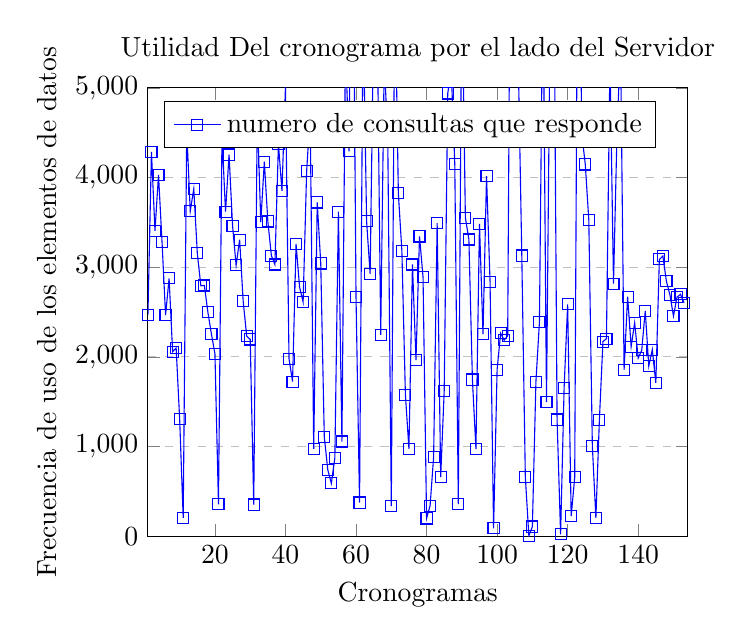
\begin{tikzpicture}
\begin{axis}[
    title={Utilidad Del cronograma por el lado del Servidor},
    xlabel={Cronogramas},
    ylabel={Frecuencia de uso de los elementos de datos},
    xmin=1, xmax=154,
    ymin=0, ymax=5000,
    xtick={},
    ytick={},
    legend pos=north west,
    ymajorgrids=true,
    grid style=dashed,
]

\addplot[
    color=blue,
    mark=square,
    ]
    coordinates {
(1,2470)
(2,4285)
(3,3406)
(4,4029)
(5,3281)
(6,2466)
(7,2875)
(8,2058)
(9,2099)
(10,1303)
(11,205)
(12,4522)
(13,3625)
(14,3873)
(15,3157)
(16,2793)
(17,2796)
(18,2498)
(19,2255)
(20,2034)
(21,355)
(22,4475)
(23,3619)
(24,4256)
(25,3462)
(26,3021)
(27,3307)
(28,2623)
(29,2232)
(30,2194)
(31,353)
(32,4721)
(33,3503)
(34,4177)
(35,3510)
(36,3129)
(37,3030)
(38,4374)
(39,3852)
(40,5017)
(41,1980)
(42,1724)
(43,3256)
(44,2776)
(45,2612)
(46,4070)
(47,4710)
(48,973)
(49,3722)
(50,3042)
(51,1109)
(52,739)
(53,589)
(54,874)
(55,3620)
(56,1056)
(57,5479)
(58,4292)
(59,7795)
(60,2665)
(61,375)
(62,5900)
(63,3511)
(64,2923)
(65,5765)
(66,5793)
(67,2245)
(68,5317)
(69,4421)
(70,334)
(71,6265)
(72,3823)
(73,3183)
(74,1577)
(75,974)
(76,3030)
(77,1965)
(78,3343)
(79,2890)
(80,198)
(81,341)
(82,883)
(83,3491)
(84,659)
(85,1619)
(86,4938)
(87,5192)
(88,4155)
(89,357)
(90,6323)
(91,3553)
(92,3309)
(93,1747)
(94,970)
(95,3484)
(96,2253)
(97,4016)
(98,2837)
(99,88)
(100,1858)
(101,2263)
(102,2186)
(103,2236)
(104,8631)
(105,5516)
(106,5304)
(107,3130)
(108,661)
(109,4)
(110,107)
(111,1721)
(112,2388)
(113,6362)
(114,1495)
(115,5721)
(116,7081)
(117,1301)
(118,20)
(119,1656)
(120,2586)
(121,223)
(122,656)
(123,8152)
(124,4488)
(125,4146)
(126,3526)
(127,1010)
(128,201)
(129,1299)
(130,2170)
(131,2203)
(132,5322)
(133,2816)
(134,4514)
(135,5491)
(136,1856)
(137,2672)
(138,2114)
(139,2380)
(140,1986)
(141,2074)
(142,2513)
(143,1897)
(144,2081)
(145,1709)
(146,3087)
(147,3124)
(148,2843)
(149,2690)
(150,2455)
(151,2666)
(152,2697)
(153,2602)
    };
    \legend{numero de consultas que responde}

\end{axis}
\end{tikzpicture}

